\section{Feature 2: Blood Report Analyser}

\begin{frame}{Intelligent Biomarker Extraction}
    \begin{itemize}
        \item \textbf{Medical OCR}: Specialized parser for clinical reports (CBC, Lipid Panel, Metabolic Panel).
        \item \textbf{Biomarker Status}: Automatic detection of abnormal values against standard reference ranges.
        \item \textbf{Profile Synchronization}: Updates the user's HealthScan profile dynamically based on report findings.
        \item \textbf{Adaptive Suggestions}: Generates dietary preferences (e.g., Low-Sugar, Keto) and daily nutrient limits automatically.
    \end{itemize}
\end{frame}

\begin{frame}{Blood Report Interface}
    \begin{columns}
        \begin{column}{0.6\textwidth}
            \centering
            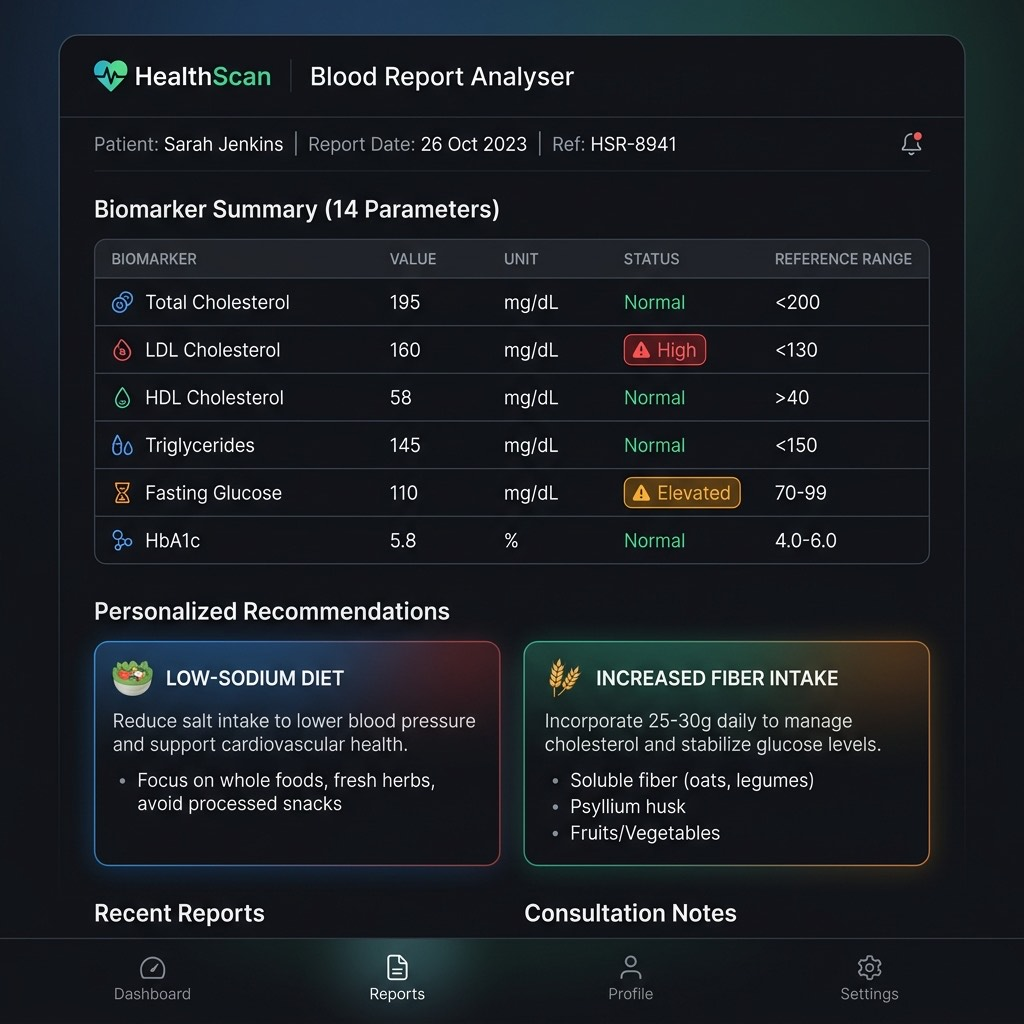
\includegraphics[width=\textwidth]{healthscan_blood_report_1777546417517.jpg}
            \captionof{figure}{Blood Report Analysis UI}
        \end{column}
        \begin{column}{0.4\textwidth}
            \textbf{Profile Updates:}
            \begin{itemize}
                \item New Condition: \texttt{Hypertension}
                \item Daily Limit: \texttt{Sodium < 2g}
                \item Recommendation: \texttt{Low-Fat Diet}
            \end{itemize}
        \end{column}
    \end{columns}
\end{frame}
